\chapter{Introduction}
\label{chapter:Introduction}

%Here starts the thesis with an introduction. Please use nice latex and bibtex entries \cite{latex}. 

%no citations in introduction
\section{Motivation}
Mobile robots are becoming a reality in everyday life.  We are already starting to see robotic lawn mowers, vacuum cleaners, robots in logistics, autonomous driving cars, mining robots, agricultural robots, underwater robots and even flying robots for a wide span of aerial tasks such as inspection, mapping or even delivery.  However unlike robots with a fixed base, or robots confined to a controlled area, mobile robots face a much more difficult problem; localization.  In order to make these new robotic applications work, robots need to have robust, reliable and cost effective localization solutions.

Localization is the ability for a robot to determine its position against a map.  The map could be known a priori, downloaded from a cloud or even generated as the robot explores, as per simultaneous localization and mapping (SLAM).  

Many localization technologies have emerged in the last 20 years.  For indoor localization a popular approach has been to use a 2D laser scanner mounted close to the ground such that is scans walls and furniture.  Using SLAM algorithms, this has proven to work well in indoor environments, however this strategy does not work outdoors, as outdoor areas have spaces too large with not enough structured obstacles to identify and localization against.

It is also possible for a robot to localize itself with respect to its starting position using odometry and inertial sensing.  However even the most accurate inertial measurement units (IMU) have bias and drift.  Odometry also suffers from drift and therefore the accuracy of the localization will deteriorate over time.

For outdoor applications Global Positioning System GPS provides latitude and longitude coordinates to an accuracy within about 10 meters.  Differential GPS (DGPS) can improve accuracy to within meters or even less by having a second fixed GPS receiver with known GPS coordinates.  This kind of accuracy is sufficient for some applications, such as agricultural robotics, or aerial navigation however it is still insufficient for applications such as autonomous driving where the accuracy needs to be within 20cm in order to stay within a lane on the road.  In addition autonomous cars need to handle GPS outages for areas with bad coverage or tunnels.  The autonomous driving cars have overcome this problem by localizing with highly accurate 360$^{\circ}$ laser scanners.  However these laser scanners are inhibitively expensive for commercial products, as well as being not reliable enough in terms of auto industry standards.

\begin{figure}[h]
  \centering
    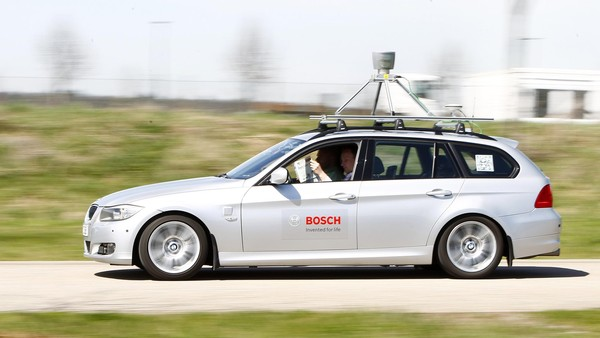
\includegraphics[width=0.77\textwidth]{chapters/images/bosch_car}
  \caption{Bosch autonomous driving car.}
  \label{fig:bosch_car}
\end{figure}

Other robotics applications, such as robotic lawn movers, farming robots or forklift robots would benefit from localization accuracy better than GPS.  There also exist other outdoor applications that have no access to GPS, such as underwater robotics or mining robots.

So despite the advances in localization technology, there is still a need for highly accurate, reliable localization.  One avenue to explore in order to tackle this need is localization with cameras.  Cameras are inexpensive and small.  There already exists a vast number of localization algorithms using cameras, as well as a strong research community.  Nevertheless cameras do have a number of clear disadvantages; input data is highly variant on lighting conditions, portions of the field of view may be easily occluded, and the vast amount of data requires significant processing to be interpreted correctly.

A number of different types of cameras exist, each having their own advantages and disadvantages.  Rather than selecting one type of camera and attempting to overcome its shortfalls, a more sound strategy would be to utilise multiple cameras simultaneously, in order to improve accuracy, robustness and reliability.  This technique of leveraging multiple sensory sources to find complimentary qualities is called sensor fusion.  Typical examples of sensor pairs include odometry/inertial, laser/inertial, and inertial/visual.  In this thesis the idea of fusing different camera types for visual localization will be explored.

\section{Problem Statement}

In this thesis fusion of stereo and omnidirectional cameras will be explored.  A number of questions with regard to this fusion will be addressed, mainly:
\begin{itemize}
 \item What is the best approach to camera fusion for improving overall accuracy and robustness?
 \item How can loop closures be identified using an omnidirectional camera?
 \item How can the scale estimation problem of registration with omni camera data be resolved by stereo data?
 \item How can a highly accurate extrinsic calibration between the cameras be achieved for use in such a system?
 \item How can a solution be integrated into an existing SLAM system?
\end{itemize}

A solution for camera fusion will be selected and implemented.  This will be integrated into an existing SLAM system.  Identifying and calculating loop closures using the omni camera will be discussed in detail.  An evaluation will be performed which will demonstrate that the method choosen considerably improves the accuracy and robustness of the existing SLAM system.  Any supporting algorithms or calibrations will also be presented in full.

\section{Outline}

This thesis is split up into chapters.  Chapter 2 will cover all the background theory and  algorithms used by this thesis, as well as outline related work.  The idea behind multiple camera fusion will be expanded on in chapter 3, along with a discussion of different approaches and justification of the selected approach. 

The SLAM system selected as the underlying framework for the camera fusion will be extensively explained in chapter 4.  Chapter 5 contains the first main contribution of this work; how to perform a highly accurate extrinsic calibration between stereo and omni cameras such that they may be used together.  Then, in chapter 6 the selected approach for camera fusion will be broken down in detail.  Having described the inner workings of the algorithms and system pipeline, chapter 7 will explore the system architecture developed to support the entire system.

Finally, chapter 8 will provide an extensive evaluation of the system, and these findings will be summarized in chapter 9.